\documentclass{standalone}
\usepackage{tikz}
\usetikzlibrary{patterns, positioning}


\begin{document}
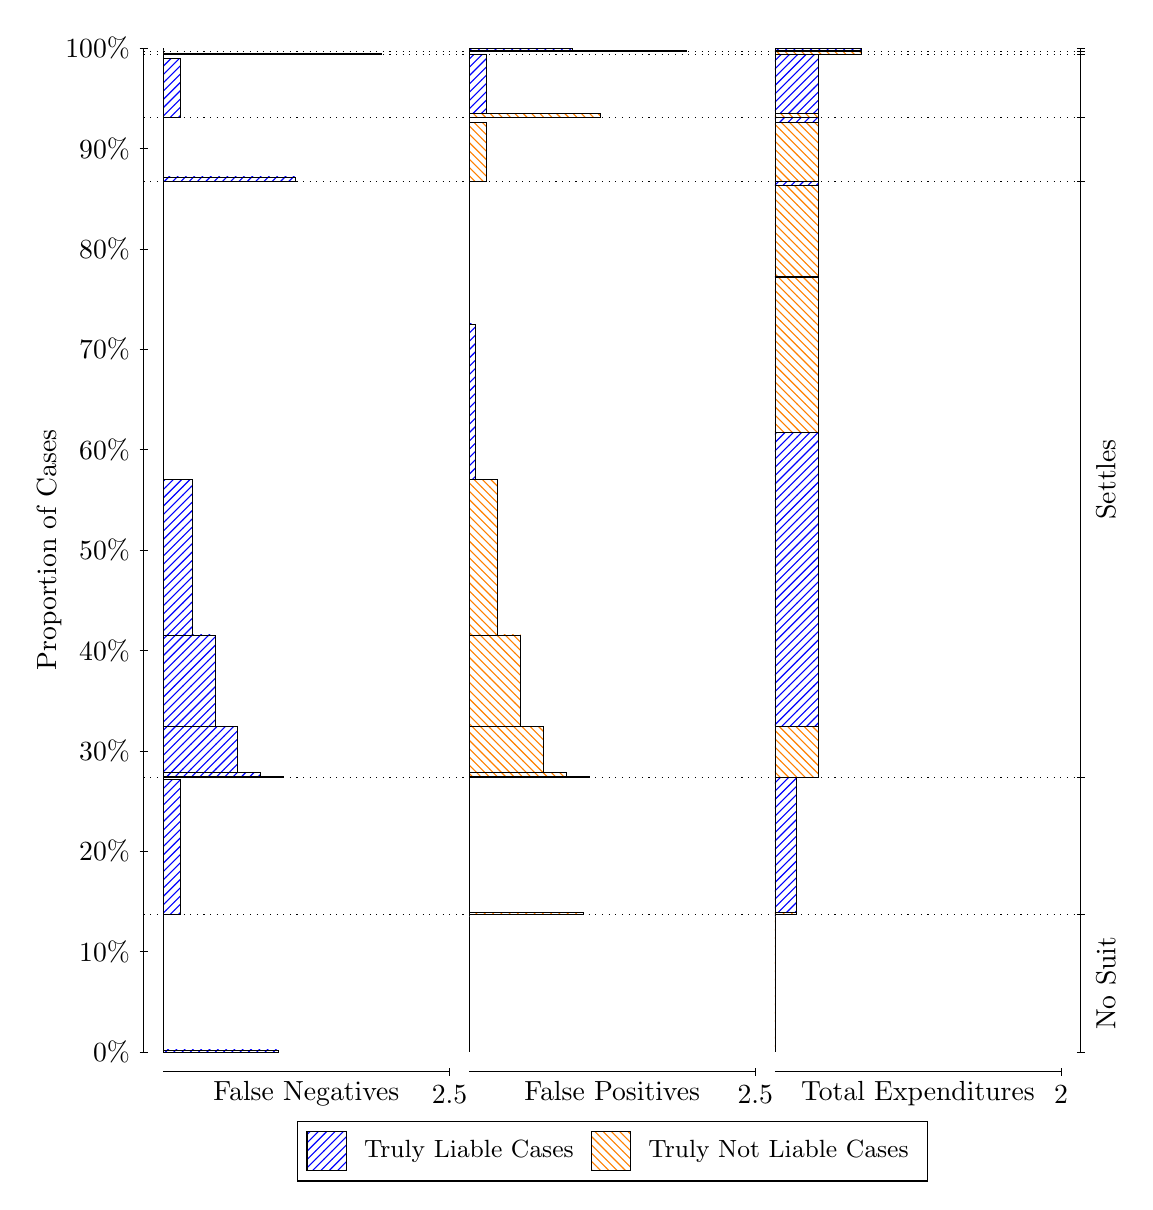
\begin{tikzpicture}
\draw[black, very thin] (1.5,1.75) -- (1.5,14.5);
\node[rotate=90, text=black, anchor=center] at (0.3, 8.125) {Proportion of Cases};
\draw[black, very thin] (1.45,1.75) -- (1.55,1.75);
\node[text=black, anchor=east] at (1.45, 1.75) {0\%};
\draw[black, very thin] (1.45,3.025) -- (1.55,3.025);
\node[text=black, anchor=east] at (1.45, 3.025) {10\%};
\draw[black, very thin] (1.45,4.3) -- (1.55,4.3);
\node[text=black, anchor=east] at (1.45, 4.3) {20\%};
\draw[black, very thin] (1.45,5.575) -- (1.55,5.575);
\node[text=black, anchor=east] at (1.45, 5.575) {30\%};
\draw[black, very thin] (1.45,6.85) -- (1.55,6.85);
\node[text=black, anchor=east] at (1.45, 6.85) {40\%};
\draw[black, very thin] (1.45,8.125) -- (1.55,8.125);
\node[text=black, anchor=east] at (1.45, 8.125) {50\%};
\draw[black, very thin] (1.45,9.4) -- (1.55,9.4);
\node[text=black, anchor=east] at (1.45, 9.4) {60\%};
\draw[black, very thin] (1.45,10.675) -- (1.55,10.675);
\node[text=black, anchor=east] at (1.45, 10.675) {70\%};
\draw[black, very thin] (1.45,11.95) -- (1.55,11.95);
\node[text=black, anchor=east] at (1.45, 11.95) {80\%};
\draw[black, very thin] (1.45,13.225) -- (1.55,13.225);
\node[text=black, anchor=east] at (1.45, 13.225) {90\%};
\draw[black, very thin] (1.45,14.5) -- (1.55,14.5);
\node[text=black, anchor=east] at (1.45, 14.5) {100\%};

\draw[black, very thin] (13.4,1.75) -- (13.4,14.5);
\draw[black, very thin] (13.35,1.75) -- (13.45,1.75);
\node[anchor=west] at (13.35, 1.75) {};
\draw[black, very thin] (13.35,3.4946) -- (13.45,3.4946);
\node[anchor=west] at (13.35, 3.4946) {};
\draw[black, very thin] (13.35,5.2376) -- (13.45,5.2376);
\node[anchor=west] at (13.35, 5.2376) {};
\draw[black, very thin] (13.35,12.807) -- (13.45,12.807);
\node[anchor=west] at (13.35, 12.807) {};
\draw[black, very thin] (13.35,13.615) -- (13.45,13.615);
\node[anchor=west] at (13.35, 13.615) {};
\draw[black, very thin] (13.35,14.423) -- (13.45,14.423);
\node[anchor=west] at (13.35, 14.423) {};
\draw[black, very thin] (13.35,14.461) -- (13.45,14.461);
\node[anchor=west] at (13.35, 14.461) {};
\draw[black, very thin] (13.35,14.5) -- (13.45,14.5);
\node[anchor=west] at (13.35, 14.5) {};

\draw[black, very thin, pattern color=blue, pattern=north east lines] (1.75,1.75) rectangle (3.2033,1.7756);
\draw[black, very thin, pattern color=orange, pattern=north west lines] (1.75,1.7756) rectangle (1.75,3.4946);
\draw[black, very thin, pattern color=blue, pattern=north east lines] (1.75,3.4946) rectangle (1.968,5.2121);
\draw[black, very thin, pattern color=orange, pattern=north west lines] (1.75,5.2121) rectangle (1.75,5.2376);
\draw[black, very thin, pattern color=blue, pattern=north east lines] (1.75,5.2376) rectangle (3.276,5.2468);
\draw[black, very thin, pattern color=blue, pattern=north east lines] (1.75,5.2468) rectangle (2.9853,5.296);
\draw[black, very thin, pattern color=blue, pattern=north east lines] (1.75,5.296) rectangle (2.6947,5.8882);
\draw[black, very thin, pattern color=blue, pattern=north east lines] (1.75,5.8882) rectangle (2.404,7.0483);
\draw[black, very thin, pattern color=blue, pattern=north east lines] (1.75,7.0483) rectangle (2.1133,9.0229);
\draw[black, very thin, pattern color=orange, pattern=north west lines] (1.75,9.0229) rectangle (1.75,12.807);
\draw[black, very thin, pattern color=blue, pattern=north east lines] (1.75,12.807) rectangle (3.4213,12.863);
\draw[black, very thin, pattern color=orange, pattern=north west lines] (1.75,12.863) rectangle (1.75,13.615);
\draw[black, very thin, pattern color=blue, pattern=north east lines] (1.75,13.615) rectangle (1.968,14.366);
\draw[black, very thin, pattern color=orange, pattern=north west lines] (1.75,14.366) rectangle (1.75,14.423);
\draw[black, very thin, pattern color=blue, pattern=north east lines] (1.75,14.423) rectangle (4.5113,14.429);
\draw[black, very thin, pattern color=orange, pattern=north west lines] (1.75,14.429) rectangle (1.75,14.461);
\draw[black, very thin, pattern color=orange, pattern=north west lines] (1.75,14.461) rectangle (1.75,14.467);
\draw[black, very thin, pattern color=blue, pattern=north east lines] (1.75,14.467) rectangle (1.75,14.5);
\draw[black, very thin, pattern color=orange, pattern=north west lines] (5.6333,1.75) rectangle (5.6333,3.469);
\draw[black, very thin, pattern color=blue, pattern=north east lines] (5.6333,3.469) rectangle (5.6333,3.4946);
\draw[black, very thin, pattern color=orange, pattern=north west lines] (5.6333,3.4946) rectangle (7.0867,3.5201);
\draw[black, very thin, pattern color=blue, pattern=north east lines] (5.6333,3.5201) rectangle (5.6333,5.2376);
\draw[black, very thin, pattern color=orange, pattern=north west lines] (5.6333,5.2376) rectangle (7.1593,5.2468);
\draw[black, very thin, pattern color=orange, pattern=north west lines] (5.6333,5.2468) rectangle (6.8687,5.2961);
\draw[black, very thin, pattern color=orange, pattern=north west lines] (5.6333,5.2961) rectangle (6.578,5.8882);
\draw[black, very thin, pattern color=orange, pattern=north west lines] (5.6333,5.8882) rectangle (6.2873,7.048);
\draw[black, very thin, pattern color=orange, pattern=north west lines] (5.6333,7.048) rectangle (5.9967,9.0216);
\draw[black, very thin, pattern color=blue, pattern=north east lines] (5.6333,9.0216) rectangle (5.706,10.996);
\draw[black, very thin, pattern color=blue, pattern=north east lines] (5.6333,10.996) rectangle (5.6333,12.807);
\draw[black, very thin, pattern color=orange, pattern=north west lines] (5.6333,12.807) rectangle (5.8513,13.558);
\draw[black, very thin, pattern color=blue, pattern=north east lines] (5.6333,13.558) rectangle (5.6333,13.615);
\draw[black, very thin, pattern color=orange, pattern=north west lines] (5.6333,13.615) rectangle (7.3047,13.671);
\draw[black, very thin, pattern color=blue, pattern=north east lines] (5.6333,13.671) rectangle (5.8513,14.423);
\draw[black, very thin, pattern color=orange, pattern=north west lines] (5.6333,14.423) rectangle (5.6333,14.456);
\draw[black, very thin, pattern color=blue, pattern=north east lines] (5.6333,14.456) rectangle (5.6333,14.461);
\draw[black, very thin, pattern color=orange, pattern=north west lines] (5.6333,14.461) rectangle (8.3947,14.467);
\draw[black, very thin, pattern color=blue, pattern=north east lines] (5.6333,14.467) rectangle (6.9413,14.5);
\draw[black, very thin, pattern color=orange, pattern=north west lines] (9.5167,1.75) rectangle (9.5167,3.469);
\draw[black, very thin, pattern color=blue, pattern=north east lines] (9.5167,3.469) rectangle (9.5167,3.4946);
\draw[black, very thin, pattern color=orange, pattern=north west lines] (9.5167,3.4946) rectangle (9.7892,3.5201);
\draw[black, very thin, pattern color=blue, pattern=north east lines] (9.5167,3.5201) rectangle (9.7892,5.2376);
\draw[black, very thin, pattern color=orange, pattern=north west lines] (9.5167,5.2376) rectangle (10.062,5.8882);
\draw[black, very thin, pattern color=blue, pattern=north east lines] (9.5167,5.8882) rectangle (10.062,9.615);
\draw[black, very thin, pattern color=orange, pattern=north west lines] (9.5167,9.615) rectangle (10.062,11.589);
\draw[black, very thin, pattern color=blue, pattern=north east lines] (9.5167,11.589) rectangle (10.062,11.598);
\draw[black, very thin, pattern color=orange, pattern=north west lines] (9.5167,11.598) rectangle (10.062,12.758);
\draw[black, very thin, pattern color=blue, pattern=north east lines] (9.5167,12.758) rectangle (10.062,12.807);
\draw[black, very thin, pattern color=orange, pattern=north west lines] (9.5167,12.807) rectangle (10.062,13.558);
\draw[black, very thin, pattern color=blue, pattern=north east lines] (9.5167,13.558) rectangle (10.062,13.615);
\draw[black, very thin, pattern color=orange, pattern=north west lines] (9.5167,13.615) rectangle (10.062,13.671);
\draw[black, very thin, pattern color=blue, pattern=north east lines] (9.5167,13.671) rectangle (10.062,14.423);
\draw[black, very thin, pattern color=orange, pattern=north west lines] (9.5167,14.423) rectangle (10.607,14.456);
\draw[black, very thin, pattern color=blue, pattern=north east lines] (9.5167,14.456) rectangle (10.607,14.461);
\draw[black, very thin, pattern color=orange, pattern=north west lines] (9.5167,14.461) rectangle (10.607,14.467);
\draw[black, very thin, pattern color=blue, pattern=north east lines] (9.5167,14.467) rectangle (10.607,14.5);
\draw[black, dotted] (1.5,3.4946) -- (13.4,3.4946);
\draw[black, dotted] (1.5,5.2376) -- (13.4,5.2376);
\draw[black, dotted] (1.5,12.807) -- (13.4,12.807);
\draw[black, dotted] (1.5,13.615) -- (13.4,13.615);
\draw[black, dotted] (1.5,14.423) -- (13.4,14.423);
\draw[black, dotted] (1.5,14.461) -- (13.4,14.461);
\draw[black, very thin] (1.75,1.5) -- (5.3833,1.5);
\node[text=black, anchor=north] at (3.5667, 1.5) {False Negatives};
\draw[black, very thin] (5.3833,1.45) -- (5.3833,1.55);
\node[text=black, anchor=north] at (5.3833, 1.45) {2.5};

\draw[black, very thin] (5.6333,1.5) -- (9.2667,1.5);
\node[text=black, anchor=north] at (7.45, 1.5) {False Positives};
\draw[black, very thin] (9.2667,1.45) -- (9.2667,1.55);
\node[text=black, anchor=north] at (9.2667, 1.45) {2.5};

\draw[black, very thin] (9.5167,1.5) -- (13.15,1.5);
\node[text=black, anchor=north] at (11.333, 1.5) {Total Expenditures};
\draw[black, very thin] (13.15,1.45) -- (13.15,1.55);
\node[text=black, anchor=north] at (13.15, 1.45) {2};

\node[text=black, centered, rotate=90] at (13.72, 2.6223) {No Suit};

\node[text=black, centered, rotate=90] at (13.72, 9.0222) {Settles};





\draw (7.449999999999999,1.5) node[draw=none] (baseCoordinate) {};
\begin{scope}[align=center]
        \matrix[scale=0.5, draw=black, below=0.5cm of baseCoordinate, nodes={draw}, column sep=0.1cm]{
            \node[rectangle, draw, minimum width=0.5cm, minimum height=0.5cm, pattern color=blue, pattern=north east lines] {}; &
            \node[draw=none, font=\small, text=black] (B) {Truly Liable Cases}; &
            \node[rectangle, draw, minimum width=0.5cm, minimum height=0.5cm, pattern color=orange, pattern=north west lines] {}; &
            \node[draw=none, font=\small, text=black] (B) {Truly Not Liable Cases}; \\
            };
\end{scope}

\end{tikzpicture}
\end{document}